\chapter{Length Chase}% by Raiyan Jamil}

\begin{linkb}
   \begin{itemize}
        \item \href{https://www.youtube.com/watch?v=_JJuNoIr_v4}{Length Chase (Raiyan)}
        \item \href{https://drive.google.com/file/d/1SWvcvf99adDs0YVglds3kCpvHxeTdLqP/view}{Things are ...} 
        \item \href{https://drive.google.com/file/d/1MocEDGQHzkW7vjUj6n6HXa_m3iBQRwmG/view}{P set} 
   \end{itemize}
\end{linkb}

\section{Ceva's and Menelaus's Theorem}

A line through a vertices connecting a point on the opposite side of a vertex is called a \textbf{cevian}.

Three cevian may concurrent or not. It is detremined my the ceva's theorem. 
\begin{theorem}[Ceva's Theorem]
Let $D,E,F$ be arbitrary points on the line $BC,CA,AB$. $AD,BE,CF$ are concurrent if and only if \[\frac{BD}{DC}\cdot \frac{CE}{EA}\cdot \frac{AF}{FB}=1.\]
\end{theorem}
\begin{figure}[ht]
\centering
	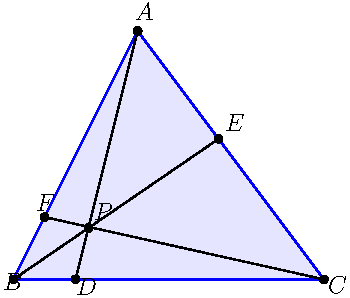
\includegraphics{ceva.pdf}
	\caption{Ceva's Theorem}
\end{figure}
You can prove the formula using areal ratios.

\begin{theorem}[Menelaus's Theorem]
Let $D,E,F$ be arbitrary points on the line $BC,CA,AB$. $D,E,F$ are collinear if and only if \[\frac{BD}{DC}\cdot \frac{CE}{EA}\cdot \frac{AF}{FB}=-1.\]
where the distances are directed.
\end{theorem}
Same as above.

\section{Trigonometric Ceva's Theorem}
\begin{theorem}[Trigonometric form of Ceva's Theorem]
Let $D,E,F$ be arbitrary points on the line $BC,CA,AB$. $AD,BE,CF$ are concurrent if and only if \[\frac{\sin \angle BAD}{\sin \angle DAC}\cdot \frac{\sin \angle CBE}{\sin \angle EBA}\cdot \frac{\sin \angle ACF}{FCB}=1.\]
\end{theorem}
For proving the formula, you have to use the fact that $\triangle ABC$ has area $=\half AB \cdot AC \sin BAC$.

\section{Isotomic Conjugate}
Let $D$ be a point on the line $BC$ and $M$ eb the midpoint o the line segment. $M'$ be the reflection of $D$ over $M$. Then, $AD'$ is called the isotomic of $AD$. 


\begin{theorem}[Isotomic Conjugate]
Let $AD,BE,CF$ are concurrent cevians of a triangle $ABC$. Then the isotomics $AD'$, $BE'$, $CF'$ are also concurrent. The point of concurrency is called the Isotomic Conjugate of the first one.
\end{theorem}

\begin{figure}[ht]
\centering
	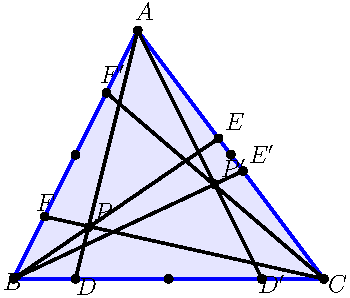
\includegraphics{isotomic.pdf}
	\caption{Isotomic conjugate $P'$.}
\end{figure}

\section{Isogonal Conjugate}
Let $AD$ be a cevian of $ABC$. Angle bisector of $\angle BAC$ is $AI$. Then, the reflection of the line $AD$ over $AI$ is called the isogonal of $AD$.
\begin{theorem}[Isogonal Conjugate]
Let $AD,BE,CF$ are concurrent cevians of a triangle $ABC$. Then the isogonals $AD',BE',CF'$ are also concurrent. The point of concurrency is called the Isogonal Conjugate of the first one.
\end{theorem}
\begin{figure}[ht]
\centering
	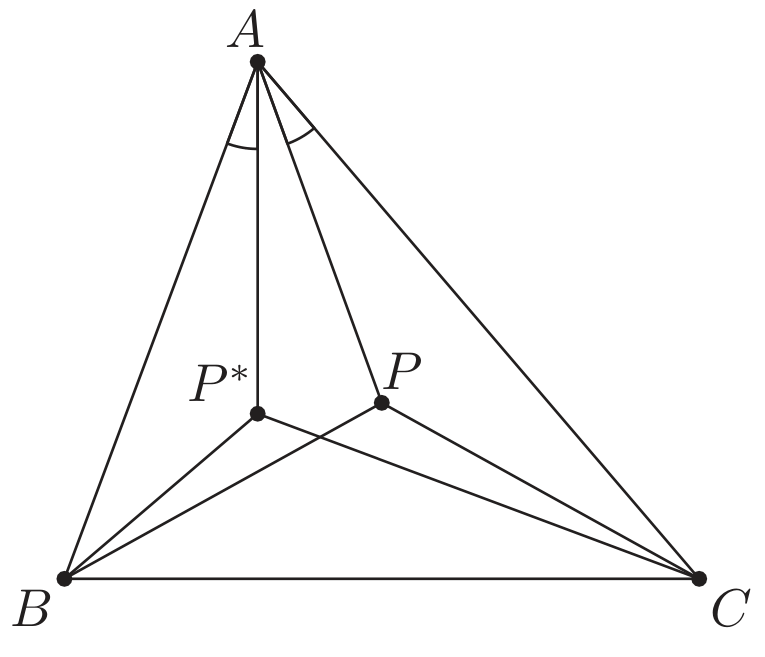
\includegraphics[scale=0.5]{isogonal-conj.png}
	\caption{Isogonal Conjugate of $P$.}
\end{figure}
\section{Projective Plane}
Here is a long discussion.

I write in a brief.

The summary of the discussion is:
\begin{enumerate}
	\ii There are infinitely many points at infinity.
	\ii There is exactly 1 line at infinity.
	\ii All points at infinity lie on the line at infinity.
\end{enumerate}
\[\mathbf{Projective \ Geometry = Euclidean \ Geometry + point \ at \ \infty + line \ at \ \infty }\]
There is an another perspective.

\textbf{Line at infinity is a circle with radius $\infty$ which goes htrough all the points at infinity.}